\section{16-bit multiplication}
\subsection{Aim}
To multiply two 16-bit numbers

\subsection{Code}
\begin{lstlisting}
DATA SEGMENT
	multiplicand DW 1000H
	multiplicator DW 200H
	product DD ?
ENDS DATA 

CODE SEGMENT
ASSUME CS:CODE, DS:DATA
START:
	MOV AX, DATA
	MOV DS, AX
	MOV AX, [multiplicand]
	MUL [multiplicator]
	MOV [product], AX
	MOV [product+2], DX
    MOV AH, 04CH
    INT 21H
ENDS CODE
END START
\end{lstlisting}

\subsection{Output}
\begin{center}
	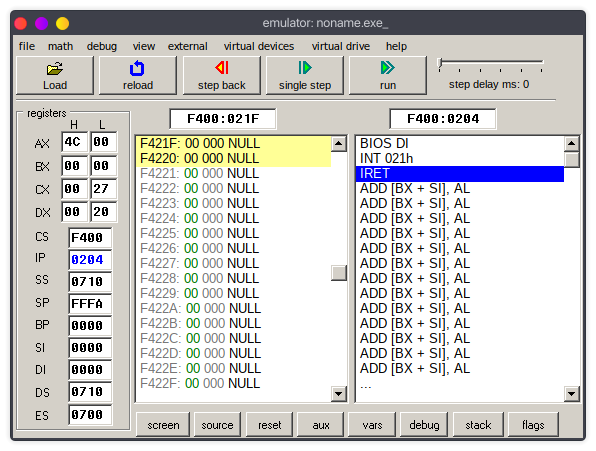
\includegraphics[width=0.90\textwidth]{img/p5/ss1.png}
	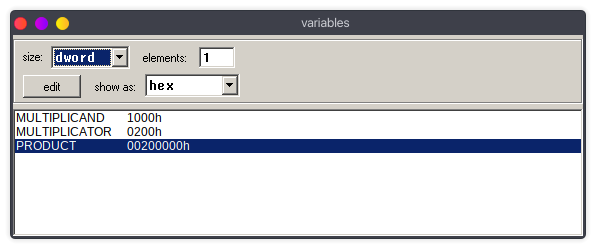
\includegraphics[width=0.90\textwidth]{img/p5/ss2.png}
\end{center}

\subsection{Result}
Two 16 bit numbers were multiplied in emu8086 and output was verified